\section{High-Level System Design}

During the requirements gathering process, four distinct components of the system were identified which form a pipeline of execution; \textit{Article Retrieval}, \textit{Keyword Extraction}, \textit{Graph Building} and \textit{Map Drawing}.

In this section, these components will be further decomposed and the flow of data between them specified. Crucially, each component will be designed to be modular, allowing both for flexible extensibility and for alternative implementations to be tested directly against each other without requiring changes to the other components.

Figure \ref{fig:dfp} outlines the decomposition of the four pipeline into their most important subtasks.

\begin{figure}[htbp!]
	\centering
	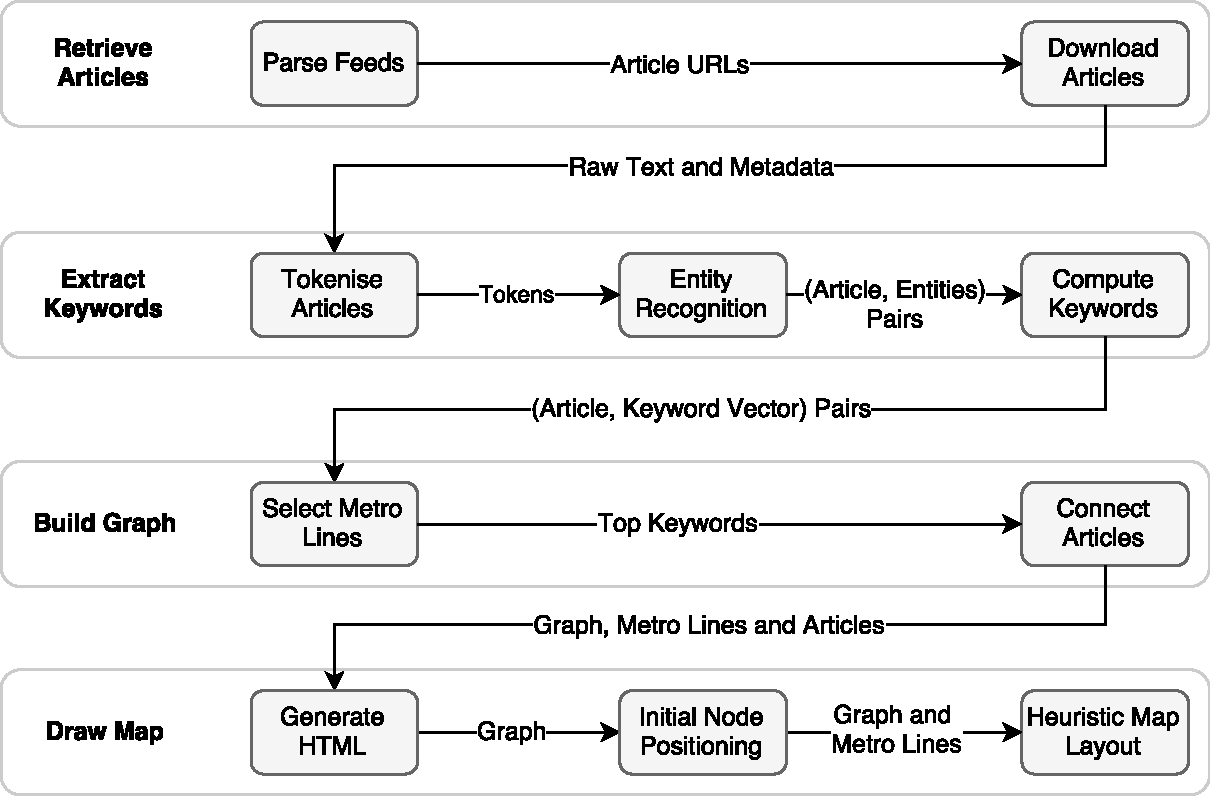
\includegraphics[width=\textwidth]{img/design/DataFlow.pdf}
	\caption{A conceptual model of data flow between components of the system.}
	\label{fig:dfp}
\end{figure}

Not included in Figure \ref{fig:dfp} is the boundary between the \textit{Build Graph} and \textit{Draw Map} stages of the pipeline, which marks the transition from the run-time Python which extracts and processes the article data, to JavaScript which only runs once the visualisation is opened in the browser; the entirety of the  \textit{Draw Map} stage. The boundary takes the form of an intermediate stage between \textit{Build Graph} and \textit{Draw Map}, where the topological map and the article data required for the visualisation are serialised to JSON\footnote{JavaScript Object Notation; http://www.json.org}.



\section{Algorithm Design}

\subsection{Keyword Extraction}

\subsection{Graph Building}

\subsection{Map Drawing}
